\documentclass[12pt,a4paper]{article}
\usepackage{ctex}
\usepackage{amsmath,amscd,amsbsy,amssymb,latexsym,url,bm,amsthm}
\usepackage{epsfig,graphicx,subfigure}
\usepackage{enumerate}
\usepackage{wrapfig}
\usepackage{mathrsfs,euscript}
\usepackage[usenames]{xcolor}
\usepackage{hyperref}
\usepackage[vlined,ruled,linesnumbered]{algorithm2e}
\hypersetup{colorlinks=true,linkcolor=black}

\newtheorem{theorem}{Theorem}
\newtheorem{lemma}[theorem]{Lemma}
\newtheorem{proposition}[theorem]{Proposition}
\newtheorem{corollary}[theorem]{Corollary}
\newtheorem{exercise}{Exercise}
\newtheorem*{solution}{Solution}
\newtheorem*{conclusion}{Conclusion}
\newtheorem{definition}{Definition}
\theoremstyle{definition}

\renewcommand{\thefootnote}{\fnsymbol{footnote}}

\newcommand{\postscript}[2]
 {\setlength{\epsfxsize}{#2\hsize}
  \centerline{\epsfbox{#1}}}

\renewcommand{\baselinestretch}{1.0}

\setlength{\oddsidemargin}{-0.365in}
\setlength{\evensidemargin}{-0.365in}
\setlength{\topmargin}{-0.3in}
\setlength{\headheight}{0in}
\setlength{\headsep}{0in}
\setlength{\textheight}{10.1in}
\setlength{\textwidth}{7in}
\makeatletter \renewenvironment{proof}[1][Proof] {\par\pushQED{\qed}\normalfont\topsep6\p@\@plus6\p@\relax\trivlist\item[\hskip\labelsep\bfseries#1\@addpunct{.}]\ignorespaces}{\popQED\endtrivlist\@endpefalse} \makeatother
\makeatletter
\renewenvironment{solution}[1][Solution] {\par\pushQED{\qed}\normalfont\topsep6\p@\@plus6\p@\relax\trivlist\item[\hskip\labelsep\bfseries#1\@addpunct{.}]\ignorespaces}{\popQED\endtrivlist\@endpefalse} \makeatother

\begin{document}
\noindent

%========================================================================
\noindent\framebox[\linewidth]{\shortstack[c]{
\Large{\textbf{Homework 09}}\vspace{1mm}\\
CS499-Mathematical Foundations of Computer Science, Jie Li, Spring 2020.}}
\begin{center}
\footnotesize{\color{blue}Name: ������ (Hongjie Fang)  \quad Student ID: 518030910150 \quad Email: galaxies@sjtu.edu.cn}
\end{center}
\section{Warmup Problems}
\begin{enumerate}
  \item [4. ] The general expansion theorem for rational functions $P(z)/Q(z)$ is not completely general, because it restricts the degree of $P$ to be less than the degree of $Q$. What happens if $P$ has a larger degree than this?
  \begin{solution}
  We can divide $P(z)$ by $Q(z)$, and get a quotient polynomial $T(z)$ and a remainder polynomial $R(z)$. The degree of remainder polynomial $R(z)$ is less than the degree of $Q(z)$, therefore we can perform general expansion theorem to rational functions $R(z) / Q(z)$. After adding $T(z)$ to the result, we expand $P(z)/Q(z)$ successfully.

  To state more formally, first we define $P(z)$ as $\sum_{i=0}^n p_i z^i$ and $Q(z)$ as $\sum_{i=0}^m q_i z^i$, and according to the problem descriptions, we have $n > m$. Therefore, we can perform polynomial division to get the quotient $T(z)$ and remainder $R(z)$, that is,
  \begin{displaymath}
  \frac{P(z)}{Q(z)} = T(z) + \frac{R(z)}{Q(z)}
  \end{displaymath}

  Then, according to the polynomial division, we know that $T(z)$ is a polynomial whose degree is $n - m$, say
  \begin{displaymath}
  T(z) = \sum_{i=0}^{n-m} t_i z^i
  \end{displaymath}

  And the degree of $R(z)$ is less than $m$, so it is also less than the degree of $Q(z)$. Thus, we perform the general expansion theorem to $R(z) / Q(z)$, and assume that we get the following expansion result.
  \begin{displaymath}
  \frac{R(z)}{Q(z)} = \sum_i r'_i z^i
  \end{displaymath}

  Therefore, we can derive the following formula (Eqn. \eqref{eq1}).
  \begin{equation}
  \begin{aligned}
  \frac{P(z)}{Q(z)} &= T(z) + \frac{R(z)}{Q(z)} \\
                    &= \sum_{i=0}^{n-m} t_i z^i + \sum_i r'_i z^i \\
                    &= \sum_i ([i \leq n-m] \cdot t_i + r'_i) z^i
  \end{aligned}
  \label{eq1}
  \end{equation}

  Hence, we expand $P(z)/Q(z)$ successfully.
  \end{solution}


  \item [5. ] Find a generating function $S(z)$ such that
  \begin{displaymath}
  [z^n]S(z) = \sum_k \binom{r}{k} \binom{r}{n-2k}
  \end{displaymath}
  \begin{solution}
  The given formula tells us an important property of $S(z)$, which is shown as follows.
  \begin{displaymath}
  \begin{aligned}
  S(z) &= \sum_n z^n \cdot \sum_k \binom{r}{k} \binom{r}{n-2k} \\
       &= \sum_n \sum_k \binom{r}{k} z^{2k} \cdot \binom{r}{n-2k} z^{n-2k} \\
       &= \sum_n \sum_k [k\textrm{ is even}]\binom{r}{\frac{k}{2}} z^{k} \cdot \binom{r}{n-k} z^{n-k} \\
       &= \left(\sum_n [n\textrm{ is even}]\binom{r}{\frac{n}{2}} z^n \right) \cdot \left(\sum_n \binom{r}{n} z^n \right) \\
       &\stackrel{\Delta}{=} F(z) \cdot G(z)
  \end{aligned}
  \end{displaymath}

  Hence, $S(z)$ is the convolution of two generating functions $F(z)$ and $G(z)$, where
  \begin{displaymath}
  \begin{aligned}
  & F(z) = \sum_n [n\textrm{ is even}]\binom{r}{\frac{n}{2}} z^n = \sum_n \binom{r}{n} z^{2n} = (1+z^2)^r \\
  & G(z) = \sum_n \binom{r}{n} z^n = (1+z)^r
  \end{aligned}
  \end{displaymath}

  Therefore, we can derive the closed form of $S(z)$ (Eqn. \eqref{eq2}).
  \begin{equation}
  S(z) = F(z) \cdot G(z) = (1+z^2)^r \cdot (1+z)^r = (1+z+z^2+z^3)^r
  \label{eq2}
  \end{equation}
  \end{solution}
\end{enumerate}

\section{Basic Problems}
\begin{enumerate}
  \item [10. ] Set $r = s = -\frac{1}{2}$ in identity (7.62) in textbook and then remove all occurrences of $\frac{1}{2}$ by using tricks like (5.36) in textbook. What amazing identity do you deduce?
  \begin{solution}
  Identity (7.62) in textbook is displayed as follows.
  \begin{displaymath}
  \sum_k \binom{r+k}{k} \binom{s+n-k}{n-k}(H_{r+k} - H_r) = \binom{r+s+n+1}{n}(H_{r+s+n+1} - H_{r+s+1})
  \end{displaymath}

  Plug $r = s = -\frac{1}{2}$ in the identity above, we can make some derivations as follows.
  \begin{displaymath}
  \begin{aligned}
  & \quad \sum_k \binom{-\frac{1}{2}+k}{k} \binom{-\frac{1}{2}+n-k}{n-k}\left(H_{-\frac{1}{2}+k} - H_{-\frac{1}{2}}\right) = \binom{n}{n}(H_{n} - H_{0}) \\
  \stackrel{(5.36)}{\Longrightarrow} & \quad \sum_k \frac{1}{2^{2k}} \binom{2k}{k} \cdot \frac{1}{2^{2(n-k)}} \binom{2(n-k)}{n-k} \cdot \left(H_{-\frac{1}{2}+k} - H_{-\frac{1}{2}}\right) = H_n \\
  \Longrightarrow & \quad 4^n H_n = \sum_k \binom{2k}{k} \binom{2n-2k}{n-k} \cdot \left( \frac{1}{k - \frac{1}{2}} + \frac{1}{k - \frac{3}{2}} + \cdots + \frac{1}{\frac{1}{2}} \right) \\
  \Longrightarrow & \quad 4^n H_n = \sum_k \binom{2k}{k} \binom{2n-2k}{n-k} \cdot 2\left( \frac{1}{2k-1} + \frac{1}{2k-3} + \cdots + \frac{1}{1} \right) \\
  \stackrel{Ex. (6.4)}{\Longrightarrow} & \quad 4^n H_n = \sum_k \binom{2k}{k} \binom{2n-2k}{n-k} \cdot \left( 2H_{2k} - H_k\right) \\
  \end{aligned}
  \end{displaymath}

  In the end, we deduce the following identity (Eqn. \eqref{eq3}).
  \begin{equation}
  4^n H_n = \sum_k \binom{2k}{k} \binom{2n-2k}{n-k} \cdot \left( 2H_{2k} - H_k\right)
  \label{eq3}
  \end{equation}
  \end{solution}


  \item [11. ] This problem, whose three parts are independent, gives practice in the manipulation of generating functions. We assuume that $A(z) = \sum_n a_nz^n$, $B(z) = \sum_n b_nz^n$, $C(z) = \sum_n c_n z^n$, and that the coefficients are zero for negative $n$.
      \begin{enumerate}[a. ]
      \item If $c_n = \sum_{j+2k\leq n}a_jb_k$, express $C$ in terms of $A$ and $B$.
      \item If $nb_n = \sum_{k=0}^n a_k \cdot \frac{2^k}{(n-k)!}$, express $A$ in terms of $B$.
      \item If $r$ is a real number and if $a_n = \sum_{k=0}^n \binom{r+k}{k} b_{n-k}$, express $A$ in terms of $B$; then use your formula to find coefficient $f_k(r)$ such that $b_n = \sum_{k=0}^n f_k(r) a_{n-k}$.
      \end{enumerate}
  \begin{solution} Here are the solutions to the sub-problems.
  \begin{enumerate}[a. ]
  \item We can derive $C(z)$ as follows.
  \begin{displaymath}
  \begin{aligned}
  C(z) &= \sum_n c_n z^n \\
       &= \sum_n z^n \cdot \sum_{j+2k \leq n} a_j b_k\\
       &= \sum_n z^n \cdot \sum_{n'=0}^n \left(\sum_{j+2k = n'} a_j b_k\right) \\
       &= \sum_n \sum_{n'=0}^n \left(z^{n'} \sum_{j+2k = n'} a_j b_k\right) \cdot \left(z^{n - n'} \cdot 1 \right) \\
       &= \left(\sum_n z^n \sum_{j+2k = n} a_j b_k \right) \cdot \left(\sum_n z^n \cdot 1 \right) \\
       &= \left(\sum_n \sum_j \left(a_jz^j\right) \cdot \left([n-j \textrm{ is even}] \cdot b_{\frac{n-j}{2}} z^{n-j}\right) \right) \cdot \frac{1}{1-z} \\
       &= \left(\sum_n a_nz^n\right) \cdot \left(\sum_n [n \textrm{ is even}] \cdot b_{\frac{n}{2}} z^n\right) \cdot \frac{1}{1-z} \\
       &= A(z) \cdot \left(\sum_n \cdot b_n z^{2n}\right)\cdot \frac{1}{1-z} \\
       &= \frac{A(z)B(z^2)}{1-z}
  \end{aligned}
  \end{displaymath}
  Therefore, we can express $C(z)$ in terms of $A(z)$ and $B(z)$ as follows (Eqn. \eqref{eq4}).
  \begin{equation}
  C(z) = \frac{A(z)B(z^2)}{1-z}
  \label{eq4}
  \end{equation}

  \item First we multiply the both sides of the equation by $z^n$, and we add a summation on $n$ to both sides, then we can get the following formula.
  \begin{displaymath}
  \sum_n nb_n z^n = \sum_n z^n \sum_{k=0}^n a_k \cdot \frac{2^k}{(n-k)!}
  \end{displaymath}
  The left side of the formula above can be rewritten as follows using the differentiate formula.
  \begin{displaymath}
  \sum_n nb_n z^n = z \sum_n b_n \cdot (nz_{n-1}) = z \sum_n b_n (z_n)' = z B'(z)
  \end{displaymath}
  Therefore, we can continue our derivations as follows.
  \begin{displaymath}
  \begin{aligned}
  z B'(z) &= \sum_n z^n \sum_{k=0}^n a_k \cdot \frac{2^k}{(n-k)!} \\
          &= \sum_n \sum_{k=0}^n \left(a_k 2^k \cdot z^k\right) \cdot \left(\frac{1}{(n-k)!} \cdot z^{n-k}\right) \\
          &= \left(\sum_n a_n 2^n \cdot z^n\right) \cdot \left(\sum_n \frac{1}{n!} \cdot z^n\right) \\
          &= \left(\sum_n a_n (2z)^n \right) \cdot e^z \\
          &= e^z A(2z)
  \end{aligned}
  \end{displaymath}
  Therefore, we can express $A(z)$ in terms of $B(z)$ as follows (Eqn. \eqref{eq5}).
  \begin{equation}
  A(z) = \frac{z}{2} e^{-\frac{z}{2}} B'\left(\frac{z}{2}\right)
  \label{eq5}
  \end{equation}

  \item We can derive $A(z)$ as follows.
  \begin{displaymath}
  \begin{aligned}
  A(z) &= \sum_n a_n z^n \\
       &= \sum_n z^n \cdot \sum_{k=0}^n \binom{r+k}{k} b_{n-k} \\
       &= \sum_n \sum_{k=0}^n \left(\binom{r+k}{k} \cdot z^k \right) \cdot \left(b_{n-k} \cdot z^{n-k}\right) \\
       &= \left(\sum_n \binom{r+n}{n} z^n \right) \cdot \left(\sum_n b_n z^n\right) \\
       &= \frac{B(z)}{(1-z)^{r+1}}
  \end{aligned}
  \end{displaymath}
  Therefore, we can express $A(z)$ in terms of $B(z)$ as follows (Eqn. \eqref{eq6}).
  \begin{equation}
  A(z) = \frac{B(z)}{(1-z)^{r+1}}
  \label{eq6}
  \end{equation}

  Hence, we can also express $B(z)$ in terms of $A(z)$ as follows.
  \begin{displaymath}
  B(z) = (1-z)^{r+1}A(z)
  \end{displaymath}
  We can unfold the generating function into summation forms, then we can make the following derivations.
  \begin{displaymath}
  \begin{aligned}
  \sum_n b_n z^n &= (1-z)^{r+1} \cdot \left(\sum_n a_n z^n \right) \\
                 &= \left(\sum_n \binom{r+1}{n} (-1)^n z^n \right) \cdot \left(\sum_n a_n z^n \right) \\
                 &= \sum_n \sum_k \left(\binom{r+1}{k} (-1)^k \cdot z^k \right) \cdot \left(a_{n-k} \cdot z^{n-k}\right) \\
                 &= \sum_n z^n \cdot \sum_k (-1)^k \binom{r+1}{k}a_{n-k}
  \end{aligned}
  \end{displaymath}
  Therefore, the corresponding coefficient must be the same, that is,
  \begin{displaymath}
  b_n = \sum_k (-1)^k \binom{r+1}{k}a_{n-k}
  \end{displaymath}
  Hence, we can get the coefficient $f_k(r)$ as follows (Eqn. \eqref{eq7}).
  \begin{equation}
  f_k(r) = (-1)^k \binom{r+1}{k}
  \label{eq7}
  \end{equation}
  \end{enumerate}
  \end{solution}
\end{enumerate}

\section{Homework Exercises}
\begin{enumerate}
  \item [22. ] \textbf{(Bonus Problem)} Let $P$ be the sum of all ways to "triangulate" polygons.
    \begin{figure}[htbp]
      \centering
      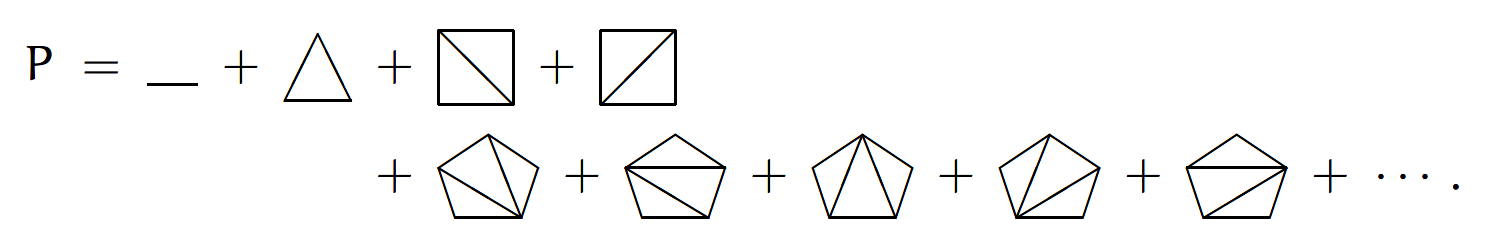
\includegraphics[width=5.5in]{ex22.png}\\
    \end{figure}

    (The first term represents a degenerate polygon with only two vertices, every other term shows a polygon that has been divided into triangles. For example, a pentagon can be triangulated in five ways.) Define a "multiplication" operation $A\Delta B$ on triangulated polygons $A$ and $B$ so that the equation
    \begin{figure}[htbp]
      \centering
      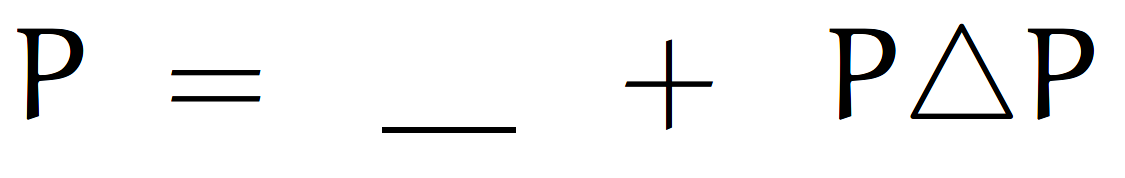
\includegraphics[width=1.5in]{ex22-2.png}\\
    \end{figure}

    is valid. Then replace each triangle by $z$; what does this tell you about the number of ways to decompose a $n$-gon into triangles?
    \begin{solution}
    We define the base of each polygon as the line segment at the bottom. If $A$ and $B$ are triangulated polygons, we can define $A \triangle B$ as the result of pasting the base of $A$ to the upper left diagonal of $\triangle$, and pasting the base of $B$ to the upper right diagonal of $\triangle$ (Notice the $\triangle$ here means both an operator and a triangle).
    \clearpage
    Here are some examples of the operator $\Delta$.
    \begin{figure}[htbp]
      \centering
      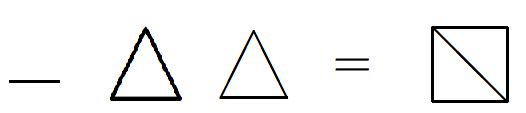
\includegraphics[width=1.5in]{ex22-3.png}\\
    \end{figure}
    \begin{figure}[htbp]
      \centering
      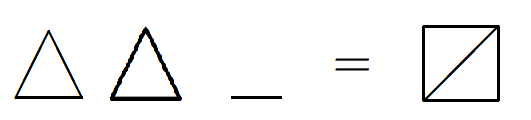
\includegraphics[width=1.5in]{ex22-4.png}\\
    \end{figure}

    Notice we re-shape the result polygons to make it look better.

    Every triangulation can be constructed uniquely in this way, because the base line is part of a unique triangle $\triangle$, and triangulated polygon $A$ and $B$ are at its left and right.

    If we replace triangle $\triangle$ by $z$, then we can get a power series $P(z)$, which can be also regarded as a generating function. The coefficient of $z^n$ in the power series is the number of triangulations with $n$ triangles, which is also the number of ways to decompose $(n+2)$-gon into triangles. And we can get the following equation (Eqn. \eqref{eq8}) according to the previous derivations.
    \begin{equation}
    P(z) = 1 + z P^2(z)
    \label{eq8}
    \end{equation}

    Therefore, we can solve $P(z)$.
    \begin{displaymath}
    P(z) = \frac{1 \pm \sqrt{1-4z}}{2z}
    \end{displaymath}

    When $z = 0$, $P(0)$ should be a finite number, therefore we must choose the substraction sign according to \underline{the L'Hospital Law}, or $P(z)$ will be an infinite number. Therefore,
    \begin{displaymath}
    P(z) = \frac{1 - \sqrt{1 - 4z}}{2z}
    \end{displaymath}

    We can expand $\sqrt{1 - 4z}$ as follows using \underline{the general binomial theorem}.
    \begin{displaymath}
    \sqrt{1-4z} = \sum_n \binom{\frac{1}{2}}{n} (-4z)^n
    \end{displaymath}

    Hence, we can continue our derivations of $P(z)$.
    \begin{displaymath}
    \begin{aligned}
    P(z) &= \frac{1 - \sqrt{1 - 4z}}{2z} \\
         &= \frac{1 - \sum_n \binom{\frac{1}{2}}{n} (-4z)^n}{2z} \\
         &= \frac{1 - \sum_n \frac{(-1)^{n-1} (2n-2)!}{2^{2n-1} n! (n-1)!} (-4z)^n}{2z} \\
         &= \sum_n \frac{(2n)!}{n!(n+1)!} z^n \\
         &= \sum_n \frac{\binom{2n}{n}}{n+1} z^n
    \end{aligned}
    \end{displaymath}

    Therefore, the number of ways to decompose a $n$-gon into triangles, which is named $p_n$ here, is as follows (Eqn. \eqref{eq9}).
    \begin{equation}
    p_n = \frac{\binom{2n}{n}}{n+1}
    \label{eq9}
    \end{equation}

    Actually, $\{p_n\}$ is actually the famous \textbf{Catalan Numbers}.

    Therefore, the number of ways to decompose $n$-gon into triangles is $p_{n-2}$, which is
    \begin{displaymath}
    \frac{\binom{2n-4}{n-2}}{n-1}
    \end{displaymath}
    \end{solution}

  \item [23. ] \textbf{(Bonus Problem)} In how many ways can a $2 \times 2 \times n$ pillar be built out of $2 \times 1 \times 1$ bricks?
  \begin{solution}
  Let $a_n$ denote the number of ways to build a $2 \times 2 \times n$ pillar using $2 \times 1 \times 1$ bricks.

  Let $b_n$ denote the number of ways to build a $2 \times 2 \times n$ pillar with a $2 \times 1 \times 1$ notch missing on the top layer.

  If $n$ is negative, then we specially define $a_n = 0$ and $b_n = 0$. Notice an important thing is, when we consider about $b_n$, we \underline{take the direction of the missing notch into account}, that is, we regard the following four situations of different directions (Fig. \ref{fig23-1}) as four different ways when counting $b_n$.

    \begin{figure}[htbp]
      \centering
      % Requires \usepackage{graphicx}
      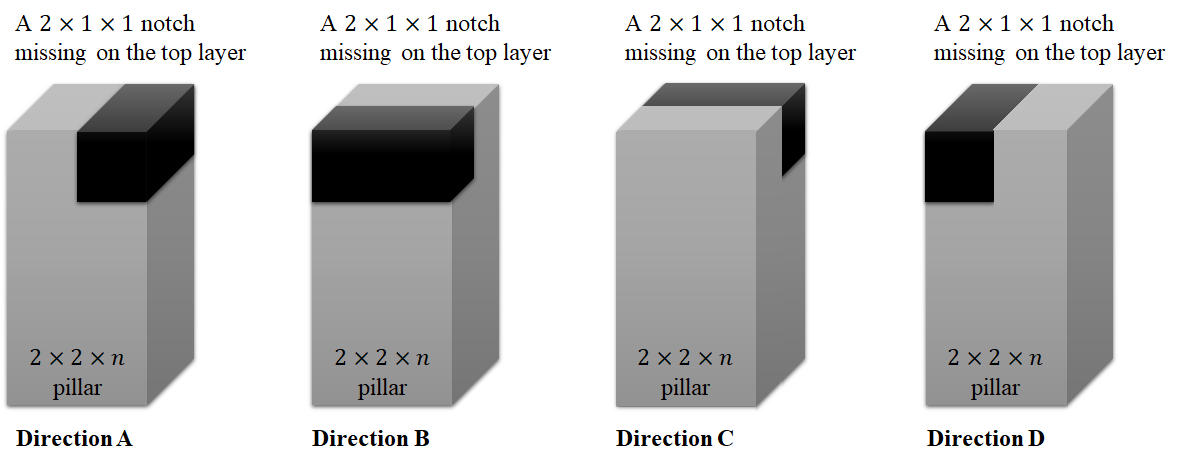
\includegraphics[width=5.3in]{ex23-1.png}\\
      \caption{Situations of different directions}\label{fig23-1}
    \end{figure}


  Therefore, there are several ways to build a $2 \times 2 \times n$ pillar.
  \begin{itemize}
  \item Add a $2 \times 2$ layer based on the $2 \times 2 \times (n-1)$ pillar, and there are two ways to add the top layer (Fig. \ref{fig23-2}).
      \begin{figure}[htbp]
      \centering
      % Requires \usepackage{graphicx}
      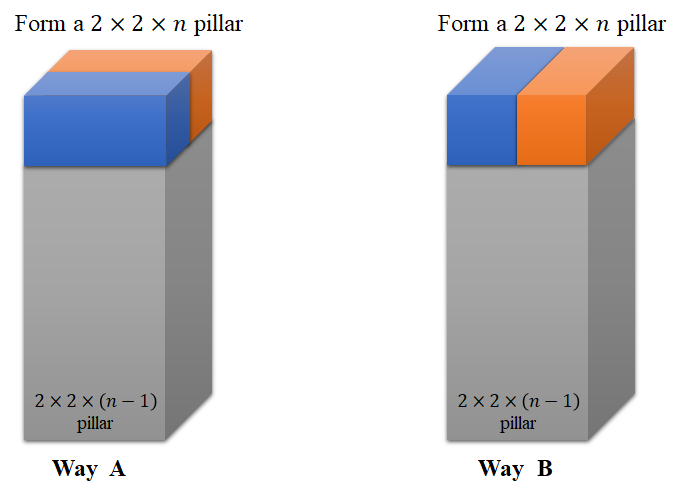
\includegraphics[width=3in]{ex23-2.png}\\
      \caption{Two ways of adding the top layer}\label{fig23-2}
    \end{figure}
  \clearpage
  \item Add three $2 \times 1 \times 1$ bricks based on the $2 \times 2 \times (n-1)$ pillar with a $2 \times 1 \times 1$ notch missing on the top layer, and there is only one way to add three bricks (Fig. \ref{fig23-3}).
      \begin{figure}[htbp]
      \centering
      % Requires \usepackage{graphicx}
      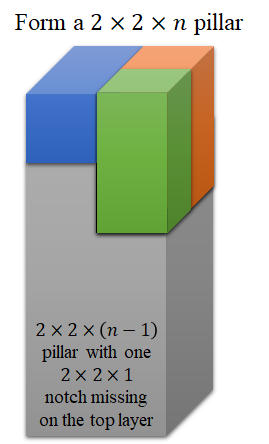
\includegraphics[width=1.4in]{ex23-3.png}\\
      \caption{One way of adding three bricks}\label{fig23-3}
    \end{figure}

    Notice here we \underline{do not allow to add a $2\times1\times1$ brick directly into the missing notch}, because we want to prevent aliases with the previous method.
  \item Add two $2 \times 2$ layers based on the $2 \times 2 \times (n-2)$ pillar using four $2 \times 2 \times 1$ bricks, and there is only one way to add four bricks (Fig. \ref{fig23-4}).
    \begin{figure}[htbp]
      \centering
      % Requires \usepackage{graphicx}
      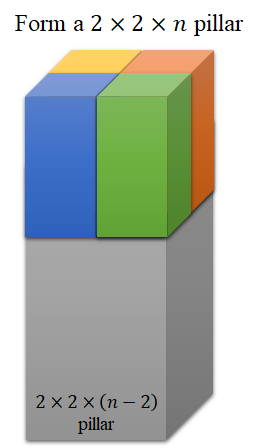
\includegraphics[width=1.4in]{ex23-4.png}\\
      \caption{One way of adding four bricks}\label{fig23-4}
    \end{figure}

    Notice here we \underline{do not allow other method to form two $2 \times 2$ layers} because we want to prevent aliases with the previous methods.
  \end{itemize}

  Notice we need to set $a_0 = 1$ because there is one way to form a null pillar. Therefore we can write down the recurrence formula of $a_n$ as follows (Eqn. \eqref{eq10}).
  \begin{equation}
  a_n = 2a_{n-1} + b_{n-1} + a_{n-2} + [n = 0]
  \label{eq10}
  \end{equation}

  Now let us consider about the construction of a $2 \times 2 \times n$ pillar with a $2 \times 1 \times 1$ notch missing on the top layer.
  \begin{itemize}
  \item An simple way is, we directly add a $2 \times 1 \times 1$ brick lying down on the top layer based on the $2 \times 2 \times (n-1)$ pillar, and there are four ways to add the brick because there are four different directions (Fig. \ref{fig23-1}).
  \clearpage
  \item Another way is, add two $2 \times 2 \times 1$ bricks based on the $2 \times 2 \times (n-1)$ pillar with a $2 \times 1 \times 1$ notch missing on the top layer. There is only one way to add the brick (Fig. \ref{fig23-5}).
  \begin{figure}[htbp]
      \centering
      % Requires \usepackage{graphicx}
      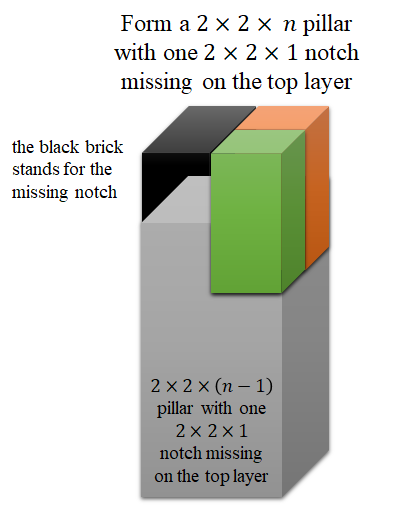
\includegraphics[width=2in]{ex23-5.png}\\
      \caption{One way of adding two bricks}\label{fig23-5}
    \end{figure}

    Notice here we \underline{do not allow other method to add two $2\times1\times1$ bricks}, because we want to prevent aliases with the previous method.
  \end{itemize}

  Therefore we can write down the recurrence formula of $b_n$ as follows (Eqn. \eqref{eq11}).
  \begin{equation}
  b_n = 4a_{n-1} + b_{n-1}
  \label{eq11}
  \end{equation}

  Suppose the generating function of $\{a_n\}$ and $\{b_n\}$ are $A(z)$ and $B(z)$ respectively. According to Equation \eqref{eq10} and Equation \eqref{eq11}, we can write the relations between the $A(z)$ and $B(z)$ as follows (Eqn. \eqref{eq12}).
  \begin{equation}
  \left\{
  \begin{aligned}
  & A(z) = 2zA(z) + zB(z) + z^2A(z) + 1 \\
  & B(z) = 4zA(z) + zB(z)
  \end{aligned}
  \right.
  \label{eq12}
  \end{equation}

  Solve the equation, and we can get the closed form of $A(z)$ as follows (Eqn. \eqref{eq13}).
  \begin{equation}
  A(z) = \frac{1-z}{1-3z-3z^2+z^3} = \frac{1-z}{(1+z)(1-4z+z^2)}
  \label{eq13}
  \end{equation}

  We can use the general partial fraction expansion method to solve the problem. We can rewrite $A(z)$ as follows.
  \begin{displaymath}
  A(z) = \frac{1-z}{(1+z)(1-4z+z^2)} = \frac{1}{3} \cdot \frac{1}{1+z} + \frac{2 - \sqrt 3}{6} \cdot \frac{1}{1 - (2-\sqrt 3)z} + \frac{2 + \sqrt 3}{6} \cdot \frac{1}{1 - (2+\sqrt 3)z}
  \end{displaymath}
  Therefore, we can expand $A(z)$ into summation form as follows.
  \begin{displaymath}
  \begin{aligned}
  A(z) &= \frac{1}{3} \cdot \frac{1}{1+z} + \frac{2 - \sqrt 3}{6} \cdot \frac{1}{1 - (2-\sqrt 3)z} + \frac{2 + \sqrt 3}{6} \cdot \frac{1}{1 - (2+\sqrt 3)z} \\
       &= \frac{1}{3} \sum_n (-z)^n + \frac{2 - \sqrt 3}{6} \sum_n \left((2-\sqrt 3)z\right)^n + \frac{2 + \sqrt 3}{6} \sum_n \left((2+\sqrt 3)z\right)^n \\
       &= \sum_n \left(\frac{1}{3} (-1)^n + \frac{1}{6} (2-\sqrt 3)^{n+1} + \frac{1}{6} (2+\sqrt 3)^{n+1} \right) z^n
  \end{aligned}
  \end{displaymath}
  Therefore, we can get the closed form of $a_n$ as follows (Eqn. \eqref{eq14}), which is the answer to the problem.
  \begin{equation}
  a_n = \frac{1}{3} (-1)^n + \frac{1}{6} (2-\sqrt 3)^{n+1} + \frac{1}{6} (2+\sqrt 3)^{n+1}
  \label{eq14}
  \end{equation}
  \end{solution}
\end{enumerate}
%=================== =====================================================
\end{document}
